\section{FEM--meshfree mixed--formulation with optimal constraint}

\subsection{Finite element and reproducing kernel approximations}

In the proposed mixed-formulation, the displacement is approximated using three-node, six-node triangular elements and four-node, eight-node quadrilateral elements \cite{hughes2000}. In order to flexcially adjust to let the dofs of pressure meets to be optimal, the reproducing kernel meshfree approximation is involved to approximate pressure.

In accordance with the reproducing kernel approximation, the entire domain $\Omega$ is discretized by $n_p$ meshfree points, $\{\boldsymbol x_I\}_{I=1}^{n_p}$. Each meshfree point equips a meshfree shape function $\Psi_I$ and nodal coefficient $p_I$, and the approximated pressure namely $p_h$ can be presented by:
\begin{equation}
p_h(\boldsymbol x) = \sum_{I=1}^{n_p} \Psi_I(\boldsymbol x) p_I
\end{equation}
where, in the reproducing kernel approximation framework, the shape function $\Psi_I$ is given by:
\begin{equation}\label{rkshape}
\Psi_I(\boldsymbol x) = \boldsymbol c(\boldsymbol x_I-\boldsymbol x) \boldsymbol p(\boldsymbol x_I-\boldsymbol x) \phi(\boldsymbol x_I - \boldsymbol x)
\end{equation}
in which $\boldsymbol p$ is the basis function, especially for 2D quadratic basis function, having the following form: 
\begin{equation}
\boldsymbol p(\boldsymbol x) = \{ 1, x, y, x^2, xy, y^2\}^T
\end{equation}
and $\phi$ stands for the kernel function. In this work, the traditional Cubic B-spline function with square suppot is used as the kernel function:
\begin{equation}
\phi(\boldsymbol x_I-\boldsymbol x) = \phi(s_x) \phi(s_y), \quad s_i = \frac{\Vert \boldsymbol x_I - \boldsymbol x\Vert}{\bar s_{iI}}
\end{equation}
with
\begin{equation}
\phi(s) =\frac{1}{3!} \begin{cases}
    (2-2s)^3 - 4(1-2s)^3 & s\le\frac{1}{2} \\
    (2-2s)^3 &\frac{1}{2}<s<1 \\
    0 & s> 1
\end{cases}
\end{equation}
where $\bar s_{iI}$'s are the support size towards the $i$-direction for the shape function $\Psi_I$.
The correction function $\boldsymbol c$ can be determined by the following so-call consistency condition:
\begin{equation}\label{cc1}
\sum_{I=1}^{n_p}\Psi_I(\boldsymbol x) \boldsymbol p(\boldsymbol x_I) = \boldsymbol p (\boldsymbol x)
\end{equation}
or equivalent shifted form:
\begin{equation}\label{cc2}
\sum_{I=1}^{n_p}\Psi_I(\boldsymbol x) \boldsymbol p(\boldsymbol x_I-\boldsymbol x) = \boldsymbol p (\boldsymbol 0)
\end{equation}
Substituting Eq. \ref{rkshape} into Eq. \ref{cc} leads to:
\begin{equation}\label{correction}
\boldsymbol c(\boldsymbol x_I-\boldsymbol x) = \boldsymbol A^{-1}(\boldsymbol x_I-\boldsymbol x)\boldsymbol p(\boldsymbol 0)
\end{equation}
in which $\boldsymbol A$ is namely moment matrix evaluating by:
\begin{equation}
\boldsymbol A(\boldsymbol x_I-\boldsymbol x) = \sum_{I=1}^{n_p}\boldsymbol p(\boldsymbol x_I-\boldsymbol x) \boldsymbol p^T(\boldsymbol x_I-\boldsymbol x)\phi(\boldsymbol x_I-\boldsymbol x)
\end{equation}
Taking Eq. \eqref{correction} back to Eq. \eqref{rkshape}, the final form of reproducing kernel shape function can be got as:
\begin{equation}
\Psi_I(\boldsymbol x) = \boldsymbol p^T(\boldsymbol 0) \boldsymbol A^{-1}(\boldsymbol x_I-\boldsymbol x)\phi(\boldsymbol x_I-\boldsymbol x)
\end{equation}

\subsection{Bubble mesh generator}
The proposed method embeds the optimal pressure DOFs to release the burden of volumetric locking. In order to maintain the number of pressure DOFs to be optimal, $n_p=n_c$, the Shimada method or namely bubble meshing method \cite{deberg2008} is used to generate the pressure nodes. 
In Shimada method, as shown in Figure \ref{fig:cloud}, a meshing node $\boldsymbol x_I$ is regard as a bubble with specific radius $r_I$ and mass $m_I$, the corresponding nodal location are determined by a dynamic system as follows:
\begin{equation} \label{bubble1}
    m_I \ddot{\boldsymbol x}_{I} + c_I \dot{\boldsymbol x}_I = \sum_{J=1}^{n_p} \bar{\boldsymbol f}_{IJ}
\end{equation}
where the dot notion over the $\boldsymbol x$ means to the time derivation of $\boldsymbol x$, i.e. $\dot{\boldsymbol x}_I, \ddot{\boldsymbol x}_I$ stands for the $\boldsymbol x_I$'s acceleration and velocity. 
The parameters $m_I, c_I$ dnotes mass and viscosity of the bubble at $\boldsymbol x_I$, and, for a better meshing efficiency and stability, these two parameters are obtained through \cite{dinh2017}:
\begin{equation} \label{bubble2}
    k = \frac{1.47}{2r_I}, \quad \zeta = \frac{c_I}{2\sqrt{m_I k}} = 0.7
\end{equation}
The interaction forces between adjacent bubbles $\bar{\boldsymbol f}_{IJ}$'s is given by:
\begin{equation}
\bar{\boldsymbol f}_{IJ} = \frac{\boldsymbol x_I - \boldsymbol x_J}{d_{IJ}} \bar f_{IJ}, \quad
\bar f_{IJ} =
\begin{cases}
    (1-w^4) e^{-w^4} & 0\le w= \frac{d_{IJ}}{r_I+r_J} \le 1.5 \\
    0 & w>1.5
\end{cases}
\end{equation}
where $d_{IJ} = \Vert \boldsymbol x_I - \boldsymbol x_J \Vert$ denotes the distance between $\boldsymbol x_I$ and $\boldsymbol x_J$.

Subsequently, the locations $\boldsymbol x_I$'s can be got by solve the above Eq. \eqref{bubble2} using conventional fourth-order Runge-Kutta method.

As shown in Figure. \ref{fig:cloud}, the detailed meshing steps are listed as follows: 
\begin{enumerate}
    \item Generate the elements for displacement using traditional meshing algorithm, for example Frontal-Delaunay algorithm \cite{deberg2008}, where the number of the displacement nodes is $n_u$. 
    \item Arrange the fixed pressure nodes on the boundary before locating nodes in the domain, and the bubbles of the boundary nodes should cover all boundaries to avoid the internal nodes escaping out.
    \item Place a specific number of nodes in the domain and let the total number of pressure nodes equal to optimal one based on the number of displacement nodes, i.e. $n_p = n_c(n_u)$. \label{step3}
    \item Determine the locations of the nodes generated by Step. \ref{step3} via solving Eq. \eqref{bubble1} using fourth-order Runge-Kutta method.
\end{enumerate}

\begin{figure}[!ht]
\centering
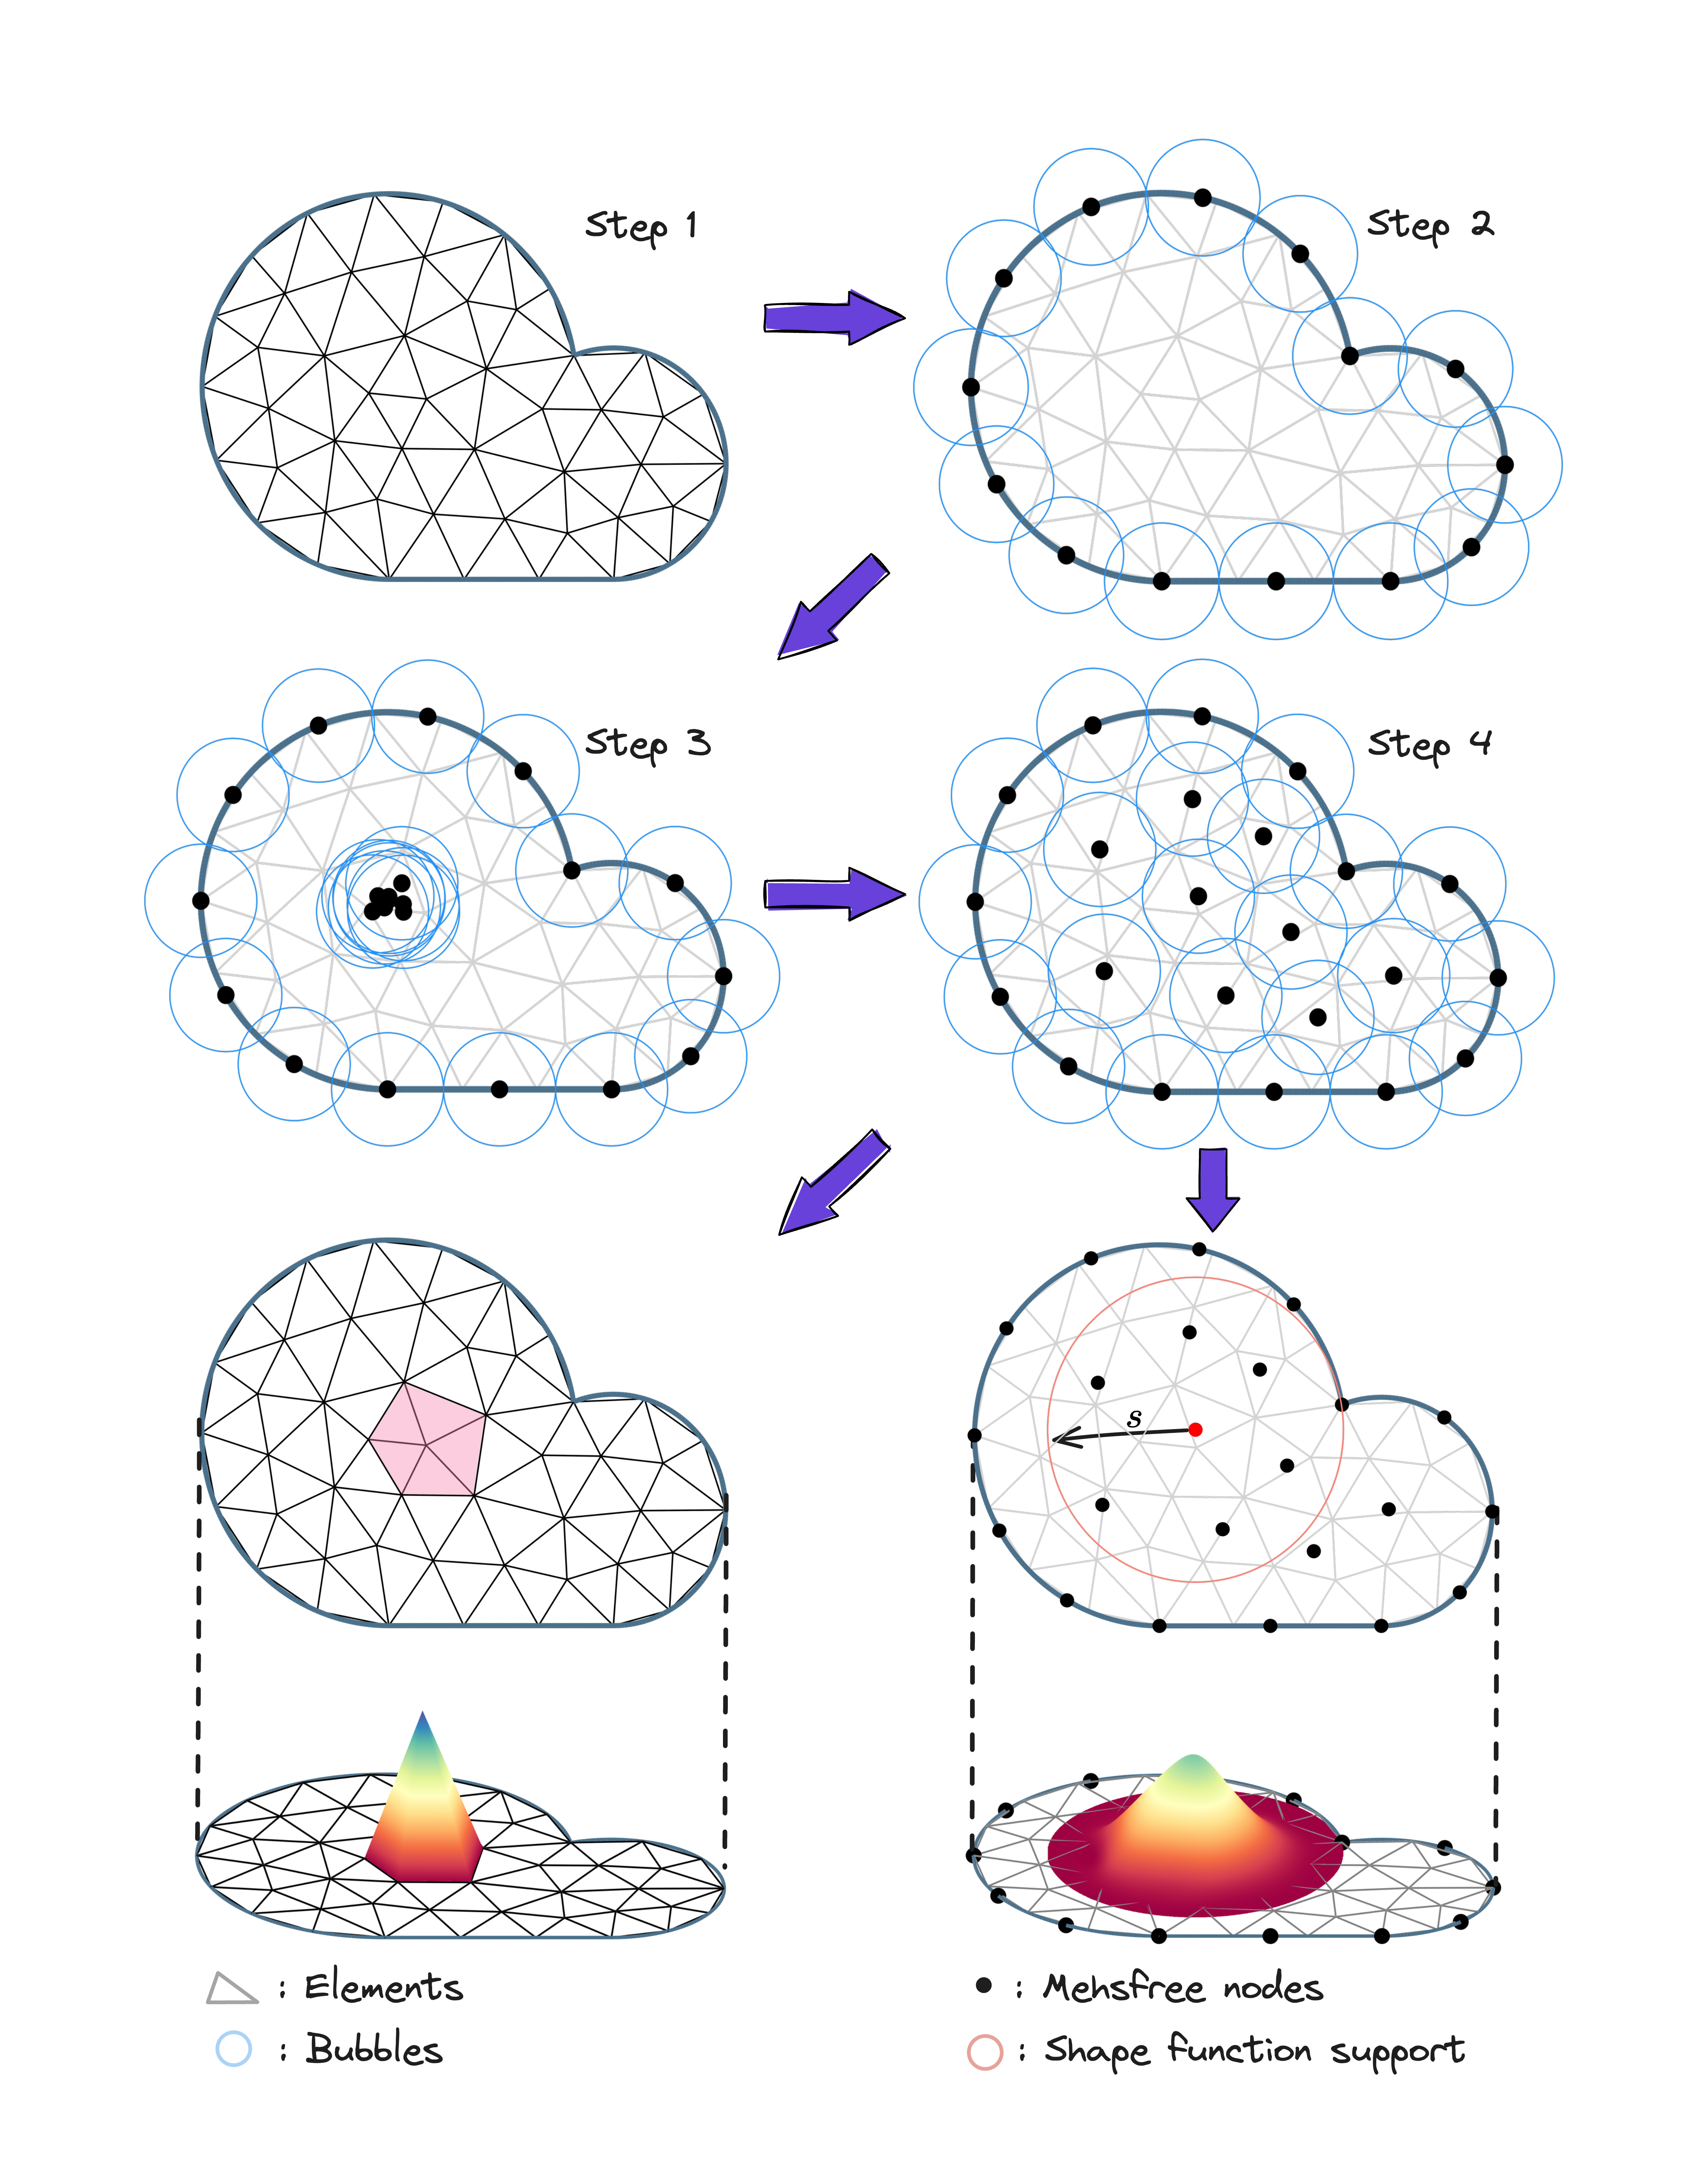
\includegraphics[width=\textwidth]{png/cloud.png}
\caption{Illustration of mesh generation for finite element and meshfree mixed approximations}\label{fig:cloud}
\end{figure}

In this mixed approximation, due to the locality of finite element shape functions and the globality of meshfree shape functions, the numerical integration for assembling the stiffness matrices is carried out in the elements of finite element approximation. 
The previous works have figured out that, the overlapping supports and the rational property of meshfree shape functions will cause a mismatch between shape function and its derivate in the procedure of the numerical integration by parts. This phenomenon, namely integration constraint, will bring the lower accurate results, and can be alleviated using higher order Gaussian quadrature rules or more efficient consistent meshfree integration rules. 
However, there is no similar problems in proposed mixed-formulations for incompressible elasticity or heat diffusion problems, since only meshfree shape functions are adopted in weak forms of Eqs. \eqref{}.
So just using the lower order Gaussian quadrature rules used in traditional finite element method can meet the accuracy requirement.
